
\chapter{The Milky Way}

\begin{figure}[h]
\vspace{-40pt}
%\begin{adjustwidth}{-2cm}{-2cm}
    \centering
    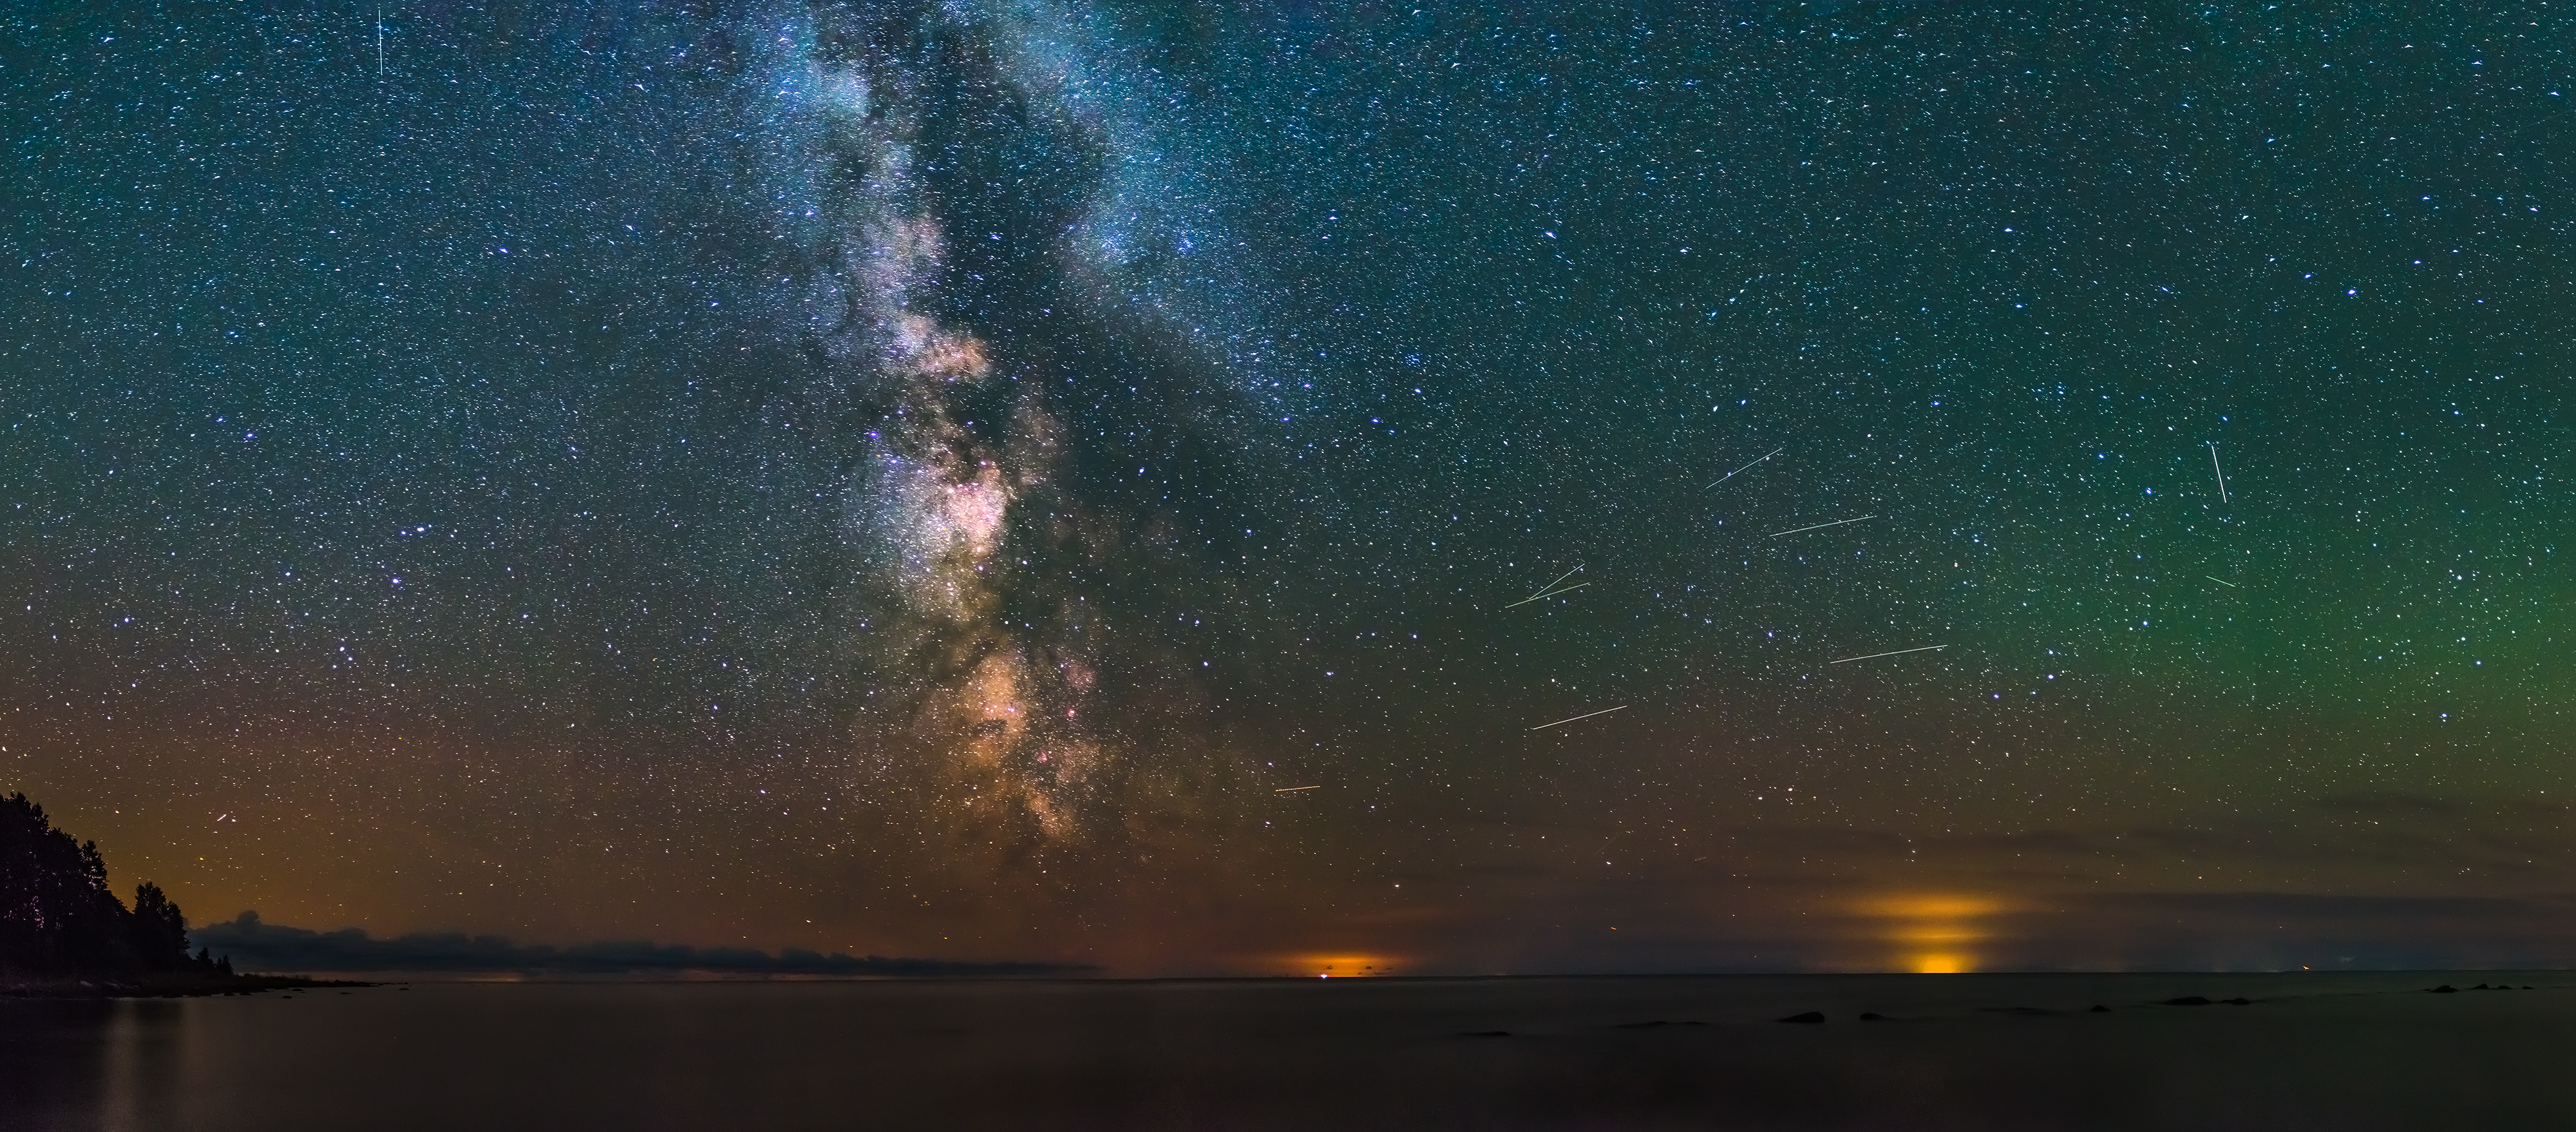
\includegraphics[width=\linewidth]{../../pictures/Linnutee_-_Milky_Way_(9)_copy.jpg}
    \caption{\footnotesize Milky Way seen from Western Estonian coast. Author:
    \href{https://commons.wikimedia.org/wiki/File:Linnutee_-_Milky_Way_(9)_copy.jpg}{Kristian Pikner}.
    License: \href{https://creativecommons.org/licenses/by-sa/4.0/deed.en}{CC-BY 4.0}}
%\end{adjustwidth}
\end{figure}
\clearpage

\lettrine[lines=4]{\goudy T}{he} breaking up of the Milky Way, of which I have just spoken, requires special notice. William Herschel, our safe and admirable guide to this portion of the regions of space, has discovered by his star gazing that the telescopic breadth of the Milky Way extends from six to seven degrees beyond what is indicated by our astronomical maps and by the extent of the sidereal radiance visible to the naked eye. The two brilliant nodes in which the branches of the zone unite, in the region of Cepheus and Cassiopeia, and in the vicinity of Scorpio and Sagittarius, appear to exercise a powerful attraction on the contiguous stars; in the most brilliant part, however, between $\alpha$ and $\gamma$ Cygni, one half of the 330,000 stars that have been discovered in a breadth of 5 are directed toward one side, and the remainder to the other. It is in this part that Herschel supposes the layer to be broken up. The number of telescopic stars in the Milky Way uninterrupted by any nebul\ae is estimated at 18 million. In order, I will not say, to realize the greatness of this number, but, at any rate, to compare it with something analogous, I will call attention to the fact that there are not in the whole heavens more than about 8000 stars, between the first and the sixth magnitudes, visible to the naked eye. The barren astonishment excited by numbers and dimensions in space, when not considered with reference to applications engaging the mental and perceptive powers of man, is awakened in both extremes of the universe, in the celestial bodies as in the minutest animalcules.\footnote{Sir John Herschel, Astronom., 624; likewise in his Observations on nebul\ae and Clusters of Stars (Phil. Transact., 1833, Part ii., p 479, fig. 25) We have here a brother system, bearing a real physical resemblance and strong analogy of structure to our own.} A cubic inch of the polishing slate of Bilin contains, according to Ehrenberg, 40,000 million of the silicious shells of Galionelle.

The stellar Milky Way, in the region of which, according to Argelander's admirable observations, the brightest stars of the firmament appear to be congregated, is almost at right angles with another Milky Way, composed of nebul\ae. The former constitutes, according to Sir John Herschel's views, an annulus, that is to say, an independent zone, somewhat remote from our lenticular-shaped starry stratum, and similar to Saturn's ring. Our planetary system lies in an eccentric direction, nearer to the region of the Cross than to the diametrically opposite point, Cassiopeia.\footnote{Sir William Herschel, in the Philos. Transact. for 1817, Part ii., p. 328. t Arago, in the Annuaire, 1842, p. 459. Sir John Herschel, in a letter from Feldhuysen, dated Jan. 13th, 1836. Nicholl, Architecture of the Heavens, 1838, p. 22. (See, also, some separate notices by Sir William Herschel on the starless space which separates us by a great distance from the Milky Way, in the Philos. Transact. for 1817, Part ii., p. 328.)} An imperfectly seen nebulous spot, discovered by Messier in 1774, appeared to present a remarkable similarity to the form of our starry stratum and the divided ring of our Milky Way.\footnote{Sir William Herschel, in the Phil. Transact. for 1785, Part i., p. 257. Sir John Herschel, Astron., 616. (The nebulous region of the heavens forms a nebulous Milky Way, composed of distinct nebul\ae, as the other of stars. The same observation was made in a letter he addressed to me in March, 1829.) Sir John Herschel, Astron., 585.}
The Milky Way composed of nebul\ae does not belong to our starry stratum, but surrounds it at a great distance without being physically connected with it, passing almost in the form of a large cross through the dense nebul\ae of Virgo, especially in the northern wing, through Coma Berenices, Ursa Major, Andromeda's girdle, and Pisces Boreales. It probably intersects the stellar Milky Way in Cassiopeia, and connects its dreary poles (rendered starless from the attractive forces by which stellar bodies are made to agglomerate into groups) in the least dense portion of the starry stratum.

We see from these considerations that our starry cluster, which bears traces in its projecting branches of having been subject in the course of time to various metamorphoses, and evinces a tendency to dissolve and separate, owing to secondary centers of attraction, is surrounded by two rings, one of which, the nebulous zone, is very remote, while the other is nearer, and composed of stars alone. The latter, which we generally term the Milky Way, is composed of nebulous stars, averaging from the tenth to the eleventh degree of magnitude, but appearing, when considered individually, of very different magnitudes, while isolated starry clusters (starry swarms) almost always exhibit throughout a character of great uniformity in magnitude and brilliancy.

In whatever part the vault of heaven has been pierced by powerful and far-penetrating telescopic instruments, stars or luminous nebul\ae are everywhere discoverable, the former, in some cases, not exceeding the twentieth or twenty-fourth degree of telescopic magnitude. A portion of the nebulous vapor would probably be found resolvable into stars by more powerful optical instruments. As the retina retains a less vivid impression of separate than of infinitely near luminous points, less strongly marked photometric relations are excited in the latter case, as Arago has recently shown.\footnote{Arago, in the Annuaire, 1842, p. 282-285, 409-411, and 439-442.} The definite or amorphous cosmical vapor so universally diffused, and which generates heat through condensation, probably modifies the transparency of the universal atmosphere, and diminishes that uniform intensity of light which, according to Halley and Olbers, should arise if every point throughout the depths of space were filled by an infinite series of stars.\footnote{Olbers, on the transparency of celestial space, in Bode's Jahr\'{e}., 1826, s. 110-121.} The assumption of such a distribution in space is, however, at variance with observation, which shows us large starless regions of space, openings in the heavens, as William Herschel terms them, one four degrees in width, in Scorpio, and another in Serpentarius. In the vicinity of both, near their margin, we find unresolvable nebul\ae, of which that on the western edge of the opening in Scorpio is one of the most richly thronged of the clusters of small stars by which the firmament is adorned. Herschel ascribes these openings or starless regions to the attractive and agglomerative forces of the marginal groups.\footnote{An opening in the heavens, William Herschel, in the Phil. Trans. for 1785, vol. lxxv., Part i., p. 256. Le Frangais Lalande, in the Connaiss. des T'ems pour l'An. VIII., p. 383. Arago, in the Annuaire, 1842, p. 425.} They are parts of our starry stratum, says he, with his usual graceful animation of style, that have experienced great devastation from time. If we picture to ourselves the telescopic stars lying behind one another as a starry canopy spread over the vault of heaven, these starless regions in Scorpio and Serpentarius may, I think, be regarded as tubes through which we may look into the remotest depths of space. Other stars may certainly lie in those parts where the strata forming the canopy are interrupted, but these are unattainable by our instruments. The aspect of fiery meteors had led the ancients likewise to the idea of clefts or openings (chasmata) in the vault of heaven. These openings were, however, only regarded as transient, while the reason for their being luminous and fiery, instead of obscure, was supposed to be owing to the translucent illuminated ether which lay beyond them.\footnote{Aristot., Meteor., ii., 5, 1. Seneca, Natur. Quest., i., 14, 2. Coelum discessisse, in Cic., de Divin., i., 43.} Derham, and even Huygens, did not appear disinclined to explain in a similar manner the mild radiance of the nebul\ae.\footnote{Arago, in the Annuaire, 1842, p. 429.}
